\documentclass[twocolumn]{aastex631}

% Packages
\usepackage{microtype}  % ALWAYS!
\usepackage{amsmath}
\usepackage{amsfonts}
\usepackage{amssymb}
\usepackage{multirow}

\definecolor{pink}{RGB}{232,132,161}
\definecolor{yellow}{RGB}{255,213,0}

\newcommand{\kc}[1]{\textcolor{yellow}{\textbf{kc: #1}} }
% \newcommand{\ecite}[1]{\textcolor{pink}{\textbf{: #1}} }
% \newcommand{\e}[1]{\textcolor{yellow}{\textbf{: #1}} }

\newcommand{\remove}[1]{\textcolor{red}{#1}}
\newcommand{\add}[1]{\textcolor{green}{#1}}

\newcommand{\mlg}{\ensuremath{M_{\rm LG}}}
\newcommand{\mmto}{\ensuremath{M_{\rm M31}}}
\newcommand{\mmw}{\ensuremath{M_{\rm MW}}}
\newcommand{\vtan}{\ensuremath{v_\textrm{tan}}}
\newcommand{\vrad}{\ensuremath{v_\textrm{rad}}}
\newcommand{\mud}{\ensuremath{\mu_\delta}}
\newcommand{\mua}{\ensuremath{\mu_\alpha^*}}
\newcommand{\bov}{\ensuremath{\boldsymbol{v}}}
\newcommand{\boldx}{\ensuremath{\boldsymbol{x}}}
\newcommand{\vtrav}{\ensuremath{\bov_{\rm travel}}}
\newcommand{\xtrav}{\ensuremath{\boldx_{\rm travel}}}
\newcommand{\pos}[2]{\ensuremath{\boldx_{\rm #1 \to #2}}}
\newcommand{\vel}[2]{\ensuremath{\bov_{\rm #1 \to #2}}}
\newcommand{\mwbary}{\ensuremath{\textrm{MW}_\textrm{bary}}}
\newcommand{\mwouter}{\ensuremath{\textrm{MW}_\textrm{halo}}}
\newcommand{\mwdisk}{\ensuremath{\textrm{MW}_\textrm{disk}}}
\newcommand{\reflabel}[1]{\ensuremath{^{\mbox{\scriptsize{#1}}}}}

% Style tweaks
% \renewcommand{\twocolumngrid}{\onecolumngrid}
% \setlength{\parindent}{1.1\baselineskip}
% \sloppy\sloppypar\raggedbottom\frenchspacing

%%%%%%%%%%%%%%%%%%%%%%%%%%%%%%%%%%%%%%%%%%%%%%%%%%%%%%%%%%%%%%%%%%%%%%%%%%%%%%%%
\shorttitle{Frequency of galaxy pairs}
\shortauthors{Chamberlain et al.}

%%%%%%%%%%%%%%%%%%%%%%%%%%%%%%%%%%%%%%%%%%%%%%%%%%%%%%%%%%%%%%%%%%%%%%%%%%%%%%%%
\graphicspath{{./}{../plots/pairs_plots/}}
% Missions
\newcommand{\project}[1]{\textsl{#1}}

% Packages / projects / programming
\newcommand{\package}[1]{\textsl{#1}}
\newcommand{\acronym}[1]{{\small{#1}}}
\newcommand{\github}{\package{GitHub}}
\newcommand{\python}{\package{Python}}
\newcommand{\astropy}{\package{Astropy}}

% Stats / probability
\newcommand{\given}{\,|\,}
\newcommand{\norm}{\mathcal{N}}
\newcommand{\pdf}{\textsl{pdf}}

% Maths
\newcommand{\dd}{\mathrm{d}}
\newcommand{\transpose}[1]{{#1}^{\mathsf{T}}}
\newcommand{\inverse}[1]{{#1}^{-1}}
\newcommand{\argmin}{\operatornamewithlimits{argmin}}
\newcommand{\mean}[1]{\left< #1 \right>}

% Non-scalar variables
\renewcommand{\vec}[1]{\ensuremath{\bs{#1}}}
\newcommand{\mat}[1]{\ensuremath{\mathbf{#1}}}

% Unit shortcuts
\newcommand{\Msun}{\ensuremath{\mathrm{M}_\odot}}
\newcommand{\Mjup}{\ensuremath{\mathrm{M}_{\mathrm{J}}}}
\newcommand{\kms}{\ensuremath{\mathrm{km}~\mathrm{s}^{-1}}}
\newcommand{\pc}{\ensuremath{\mathrm{pc}}}
\newcommand{\kpc}{\ensuremath{\mathrm{kpc}}}
\newcommand{\Mpc}{\ensuremath{\mathrm{Mpc}}}
\newcommand{\kmskpc}{\ensuremath{\mathrm{km}~\mathrm{s}^{-1}~\mathrm{kpc}^{-1}}}
\newcommand{\dayd}{\ensuremath{\mathrm{d}}}
\newcommand{\yr}{\ensuremath{\mathrm{yr}}}
\newcommand{\Myr}{\ensuremath{\mathrm{Myr}}}
\newcommand{\Gyr}{\ensuremath{\mathrm{Gyr}}}
\newcommand{\Kel}{\ensuremath{\mathrm{K}}}
\newcommand{\masyr}{\ensuremath{\mathrm{mas}~\mathrm{yr}^{-1}}}
\newcommand{\muasyr}{\ensuremath{\mu\mathrm{as}~\mathrm{yr}^{-1}}}

% Misc.
\newcommand{\bs}[1]{\boldsymbol{#1}}

% Astronomy
\newcommand{\DM}{{\rm DM}}
\newcommand{\feh}{\ensuremath{{[{\rm Fe}/{\rm H}]}}}
\newcommand{\df}{\acronym{DF}}

% TO DO
\newcommand{\todo}[1]{{\color{red} TODO: #1}}
\newcommand{\apw}[1]{{\color{blue} APW says: #1}}

% Projects
\newcommand{\gaia}{\textsl{Gaia}}
\newcommand{\gaiadr}{\textsl{Gaia}~\acronym{EDR3}}
\newcommand{\hst}{\textsl{HST}}
\newcommand{\ill}{\textsl{Illustris}}
\newcommand{\tng}{\textsl{IllustrisTNG}} 



% Affiliations
\newcommand{\affuofa}{University of Arizona, 933 N. Cherry Ave,
    Tucson, AZ 85721, USA}

%% This is the end of the preamble.  Indicate the beginning of the
%% manuscript itself with \begin{document}.

\begin{document}

\title{
  Frequency of galaxy pairs in the Illustris and Illustris TNG cosmological simulations
}

\author[0000-0001-8765-8670]{Katie~Chamberlain}
\affiliation{\affuofa}

\author[0000-0003-0715-2173]{Gurtina Besla}
\affiliation{\affuofa}


\begin{abstract}
\end{abstract}

%%%%%%%%%%%%%%%%%%%%%%%%%%%%%%%%%%%
\section{Introduction}
\label{sec:intro}


%%%%%%%%%%%%%%%%%%%%%%%%%%%%%%%%%%%
\section{Methods}
\label{sec:methods}
\begin{itemize}
  \item Introduce simulations
  \item outline selection steps
  \item dwarf pairs
  \item massive pairs
  \item include table with parameters used for pairs
  \item plots
    \begin{itemize}
      \item distribution plots
      \item counts plots
    \end{itemize}
\end{itemize}


% selection criterion
\begin{table*}[htb]
  \centering
    \begin{tabular}{lcc}
     & Dwarf Pairs & Massive Pairs \\\hline\hline
    Group Mass & $8\times10^{10} < \rm M_g < 5\times10^{11} M_\odot$ & $1\times10^{12} < \rm M_g < 4\times10^{12} M_\odot$  \\
    % Subhalo Max Mass &  &  \\
    Subhalo Current Mass & $>1\times10^{10} \Msun$ & $> 5\times10^{11} \Msun$ \\
    Primary &$1\times10^{8} < \rm M_* < 5\times10^{9} \Msun$ & $5\times10^{9} < \rm M_* < 1\times10^{11} \Msun$\\\hline
    \end{tabular}
    \caption{\label{table:mass}Selection criteria for dwarf and massive pairs.}
    \end{table*}

% equivalent snapshot table
\begin{table}[]
  \centering
  \begin{tabular}{l|cc}
    \hline \hline
   & Illustris & TNG  \\ 
  \hline
  z = 0   &   135  &   99   \\
  z = 1   &   85   &   50   \\
  z = 2   &   68   &   33   \\
  z = 3   &   60   &   25   \\
  z = 4   &   54   &   21   \\
  \hline \hline
  \end{tabular}
  \caption{\label{tab:equiv-snapshot} The snapshot number of the original \ill\ and the \tng\ simulations at redshifts $z=0-4$.}
    \end{table}


\begin{figure*}[htb]
  \centering
  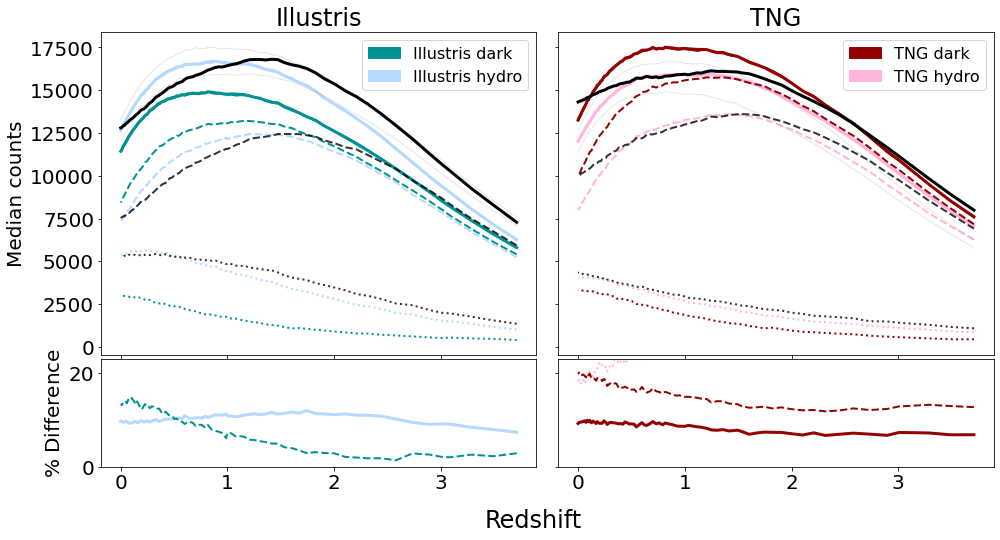
\includegraphics[width=\textwidth]{counts_dwarfs.png}
  \caption{Median counts of dwarf primaries in \ill{} and \tng{} \kc{add "dwarf" somewhere to plot}. The number of dwarf primaries peaks at $z~0.75$. TNG has higher halo count than Illustris. However, the difference between the number of halos in both dark simulations is substantial. Additionally, in Illustris, hydro halos outnumber dark halos. In TNG, the opposite is true, where dark halos outnumber hydro halos. In Illustris, this can be accounted for by the discrepant number of unpaired halos (dotted), while in TNG, the difference is dominated by pairs. 
    }
  \label{fig:counts-dwarfs}
\end{figure*}

\begin{figure*}[htb]
  \centering
  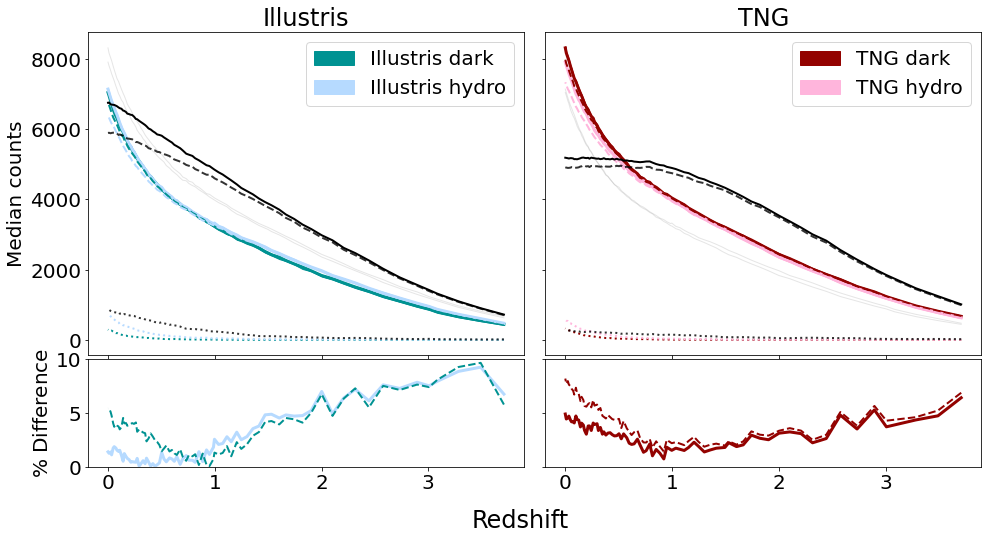
\includegraphics[width=\textwidth]{counts_massive.png}
  \caption{No turn over, instead, monotonically increasing towards a peak at low z. No significant fraction of halos that are lone subhalos. The largest differences between the hydro and dark simulations in both cases are at low z, where the counts start to diverge. TNG has a higher number of massive halos primaries than Illustris. The difference between dark and hydro is large in TNG, and at low z, the main driver of this difference is in the pairs, as opposed to the lone halos. This is not the case in Illustris, where both the pairs and unpaired halos contribute equally to the difference between dark and hydro, in opposite way! Weird… \kc{add "massive" somewhere to plot}
    }
  \label{fig:counts-massive}
\end{figure*}


%%%%%%%%%%%%%%%%%%%%%%%%%%%%%%%%%%%
\section{Results}
\label{sec:results}


%%%%%%%%%%%%%%%%%%%%%%%%%%%%%%%%%%%
\section{Discussion}
\label{sec:discussion}


%%%%%%%%%%%%%%%%%%%%%%%%%%%%%%%%%%%
\section{Summary and Conclusions}
\label{sec:summary}

%%%%%%%%%%%%%%%%%%%%%%%%
%%%%%%%%%%%%%%%%%%%%%%%%

\bibliography{refs}{}
\bibliographystyle{aasjournal}

\end{document}
